\subsection{Composition d'un API}
Un \textit{\textbf{A}utomate \textbf{P}rogrammable \textbf{I}ndustriel (\textbf{API})} est un système informatique industriel adapté aux besoins de l'industrie. Sa structure est donc similaire à celle d'un ordinateur personnel (PC) en cela qu'il est composé d'un processeur et de mémoires dédiées à des usages que nous allons développer. 

\begin{UPSTIactivite}[][Structure d'un API]
    Représenter sous forme schématique un automate industriel
    \begin{center}
        \UPSTIprofEleve{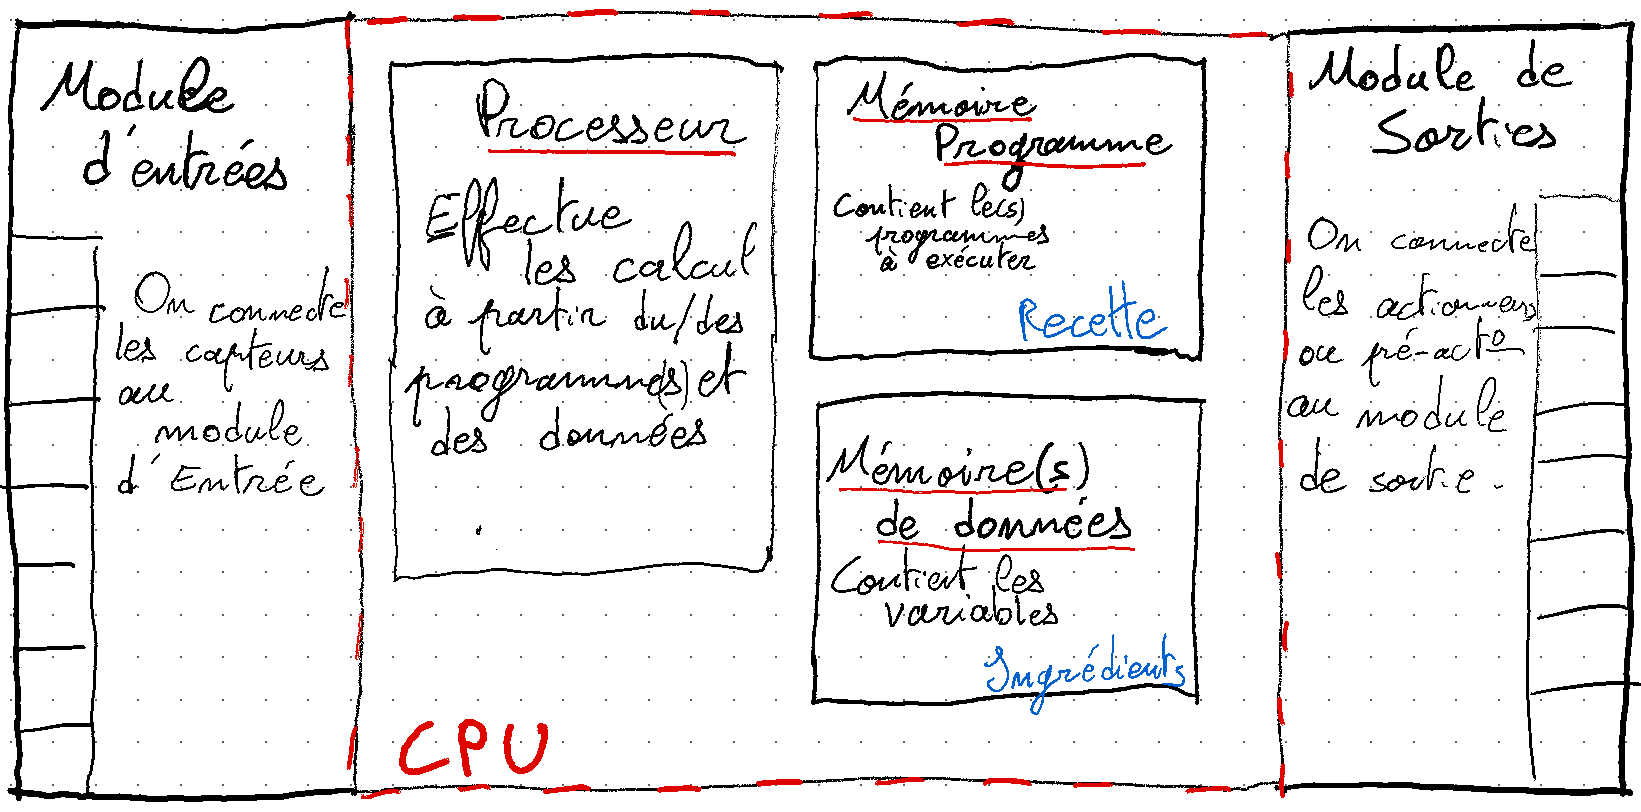
\includegraphics[height=.34\textheight]{images/API}\vspace{.06\textheight}}{\vspace{0.4\textheight}}
    \end{center}   

\end{UPSTIactivite}

\UPSTIaRetenir{%
Les \textbf{\color{red} capteurs} du système sont reliées aux \textbf{\color{red} modules d'entrées} de l'API.\\
Les \textbf{\color{green} actionneurs} et les \textbf{\color{green} pré-actionneurs}  du système sont reliées aux \textbf{\color{green} modules de sortie} de l'aPI.}


